\subsubsection{Dịch vụ cài đặt (setting service - dùng Neon Data API)}

Sử dụng Neon Data API
(REST API kết nối CSDL Postgres)
để người dùng có thể thực hiện
các yêu cầu \texttt{GET} và \texttt{POST} nhằm lưu trữ
và truy xuất các cấu hình cài đặt (dưới dạng key-value).
Kích hoạt thủ công Data API trên bảng điều khiển của Neon:

\begin{figure}[H]
\centering
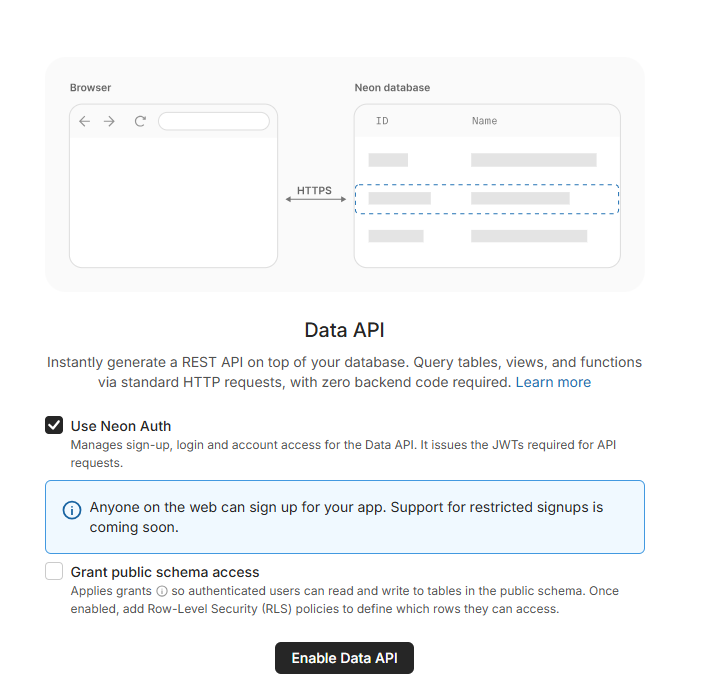
\includegraphics[width=0.65\textwidth]{pictures/setting-neonimage-1.png}
\caption{Kích hoạt thủ công Data API trên Neon}
\end{figure}

Lấy thông tin URL của REST API trên giao diện web của Neon:

\begin{figure}[H]
\centering
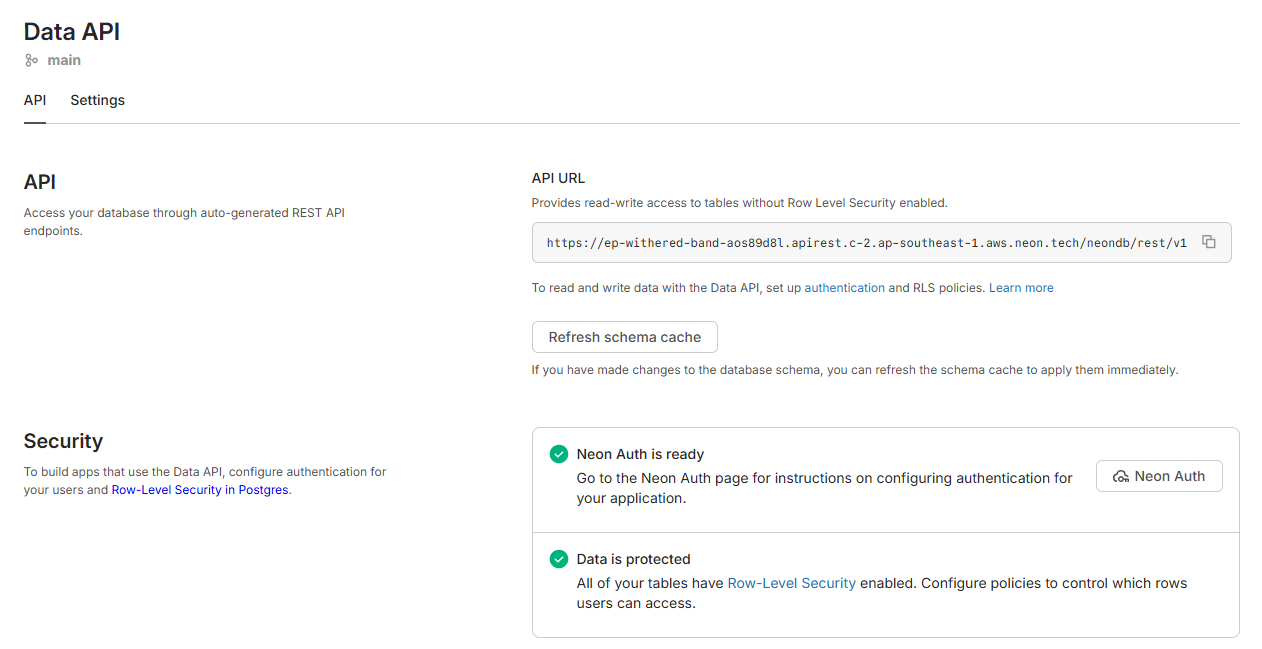
\includegraphics[width=0.95\textwidth]{pictures/setting-neonimage-2.png}
\caption{Thông tin URL REST API trên Neon}
\end{figure}

Neon hỗ trợ tích hợp cấu hình thông tin xác thực từ Supabase:

\begin{figure}[H]
\centering
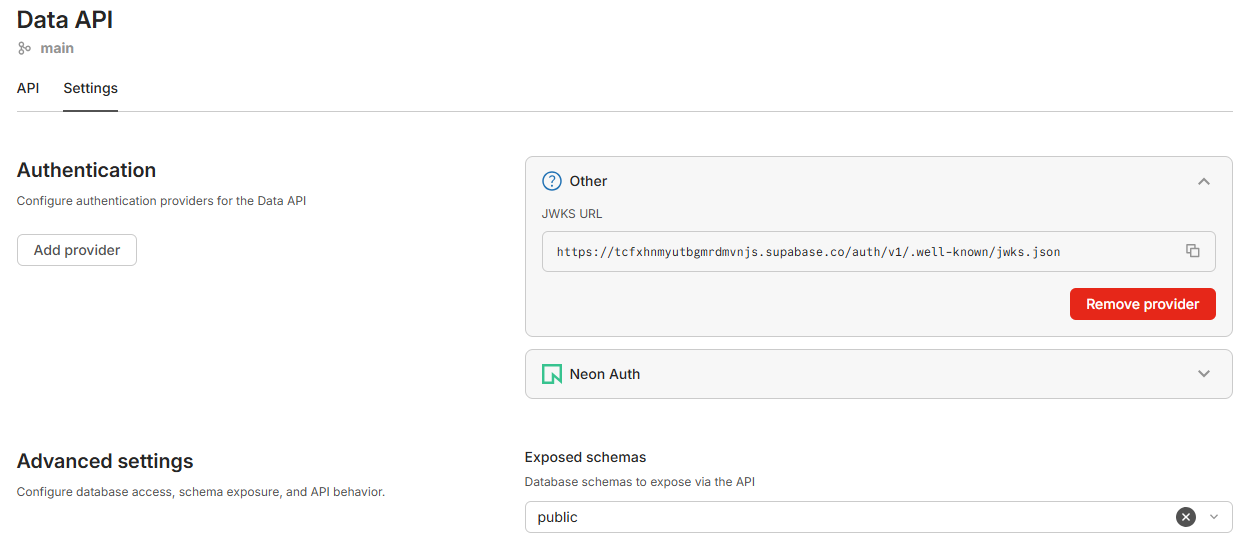
\includegraphics[width=0.95\textwidth]{pictures/setting-neonimage-3.png}
\caption{Tích hợp cấu hình xác thực Supabase trong Neon}
\end{figure}

Sử dụng SQL để tạo bảng
\texttt{settings} gồm các cột:
\texttt{id},
\texttt{user\_id},
\texttt{key},
\texttt{value}, \texttt{updated\_at}.
Kích hoạt bảo mật cấp hàng RLS (Row-Level Security) để đảm bảo chỉ chủ sở hữu mới có quyền thay đổi dữ liệu cài đặt của họ:

\begin{figure}[H]
\centering
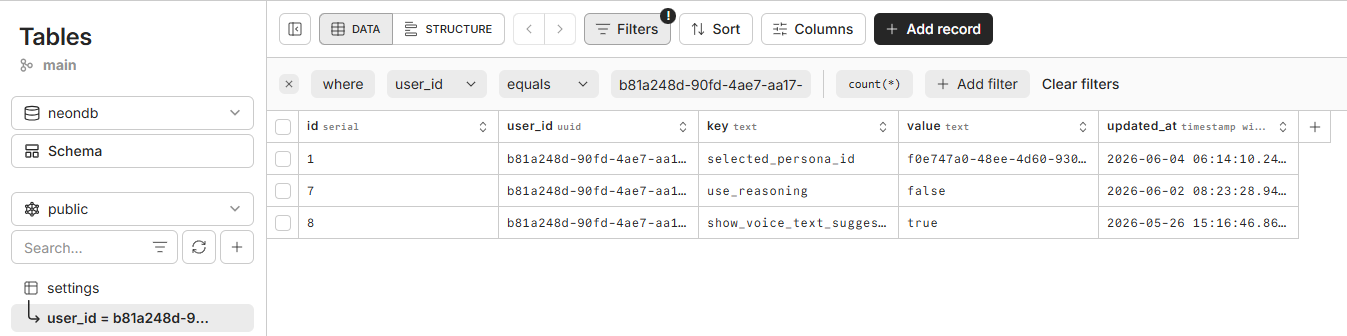
\includegraphics[width=0.95\textwidth]{pictures/setting-neonimage-6.png}
\caption{Kết quả thông tin bảng settings trên Neon}
\end{figure}

\paragraph{Cấu hình trong Kong API Gateway}

Tạo Service trong Kong trỏ trực tiếp đến endpoint REST API của bảng \texttt{settings} trên Neon.
Thay vì tạo một Route chung cho tất cả các yêu cầu,
hệ thống được cấu hình để phân loại riêng biệt luồng đọc (\texttt{GET}) và luồng ghi (\texttt{POST}).
Tham số \texttt{strip\_path=true} giúp Kong loại bỏ tiền tố URI trước khi chuyển tiếp yêu cầu đến Neon.
Cấu hình Plugin xử lý Upsert tự động:
Trong REST API dựa trên Postgres,
để thực hiện hành động Upsert
(chèn hoặc cập nhật),
client cần gửi kèm các tham số cụ thể trên URL
(\texttt{on\_conflict=user\_id,key})
và Header (\texttt{Prefer: resolution=merge-duplicates}).
Sử dụng plugin \texttt{request-transformer}
để Kong API Gateway
tự động đính kèm các tham số
và header phức tạp này trước khi gửi đến Neon.
